%%%%%%%%%%%%%%%%%%%%%%%%%%%%%%%%%%%%%%%%%%%%%%%%%%%%%%%%%%%%%%%%%
% MUW Presentation
% LaTeX Template
% Version 1.0 (27/12/2016)
%
% License:
% CC BY-NC-SA 4.0 (http://creativecommons.org/licenses/by-nc-sa/3.0/)
%
% Created by:
% Nicolas Ballarini, CeMSIIS, Medical University of Vienna
% nicoballarini@gmail.com
% http://statistics.msi.meduniwien.ac.at/
%
% Customized for UAH by:
% David F. Barrero, Departamento de Automática, UAH
%%%%%%%%%%%%%%%%%%%%%%%%%%%%%%%%%%%%%%%%%%%%%%%%%%%%%%%%%%%%%%%%%

\documentclass[10pt,compress]{beamer} % Change 10pt to make fonts of a different size
\mode<presentation>

\usepackage[spanish]{babel}
\usepackage{fontspec}
\usepackage{tikz}
\usepackage{etoolbox}
\usepackage{xcolor}
\usepackage{xstring}
\usepackage{listings}

% Introduced by David
\usepackage{eurosym}

\usetheme{UAH}
\usecolortheme{UAH}
\setbeamertemplate{navigation symbols}{} 
\setbeamertemplate{caption}[numbered]

%%%%%%%%%%%%%%%%%%%%%%%%%%%%%%%%%%%%%%%%%%%%%%%%%%%%%%%%%%%%%%%%%
%% Presentation Info
\title[Videogame engine]{Videogame engine}
\author{\asignatura\\\carrera}
\institute{}
\date{Departamento de Automática}
%%%%%%%%%%%%%%%%%%%%%%%%%%%%%%%%%%%%%%%%%%%%%%%%%%%%%%%%%%%%%%%%%


%%%%%%%%%%%%%%%%%%%%%%%%%%%%%%%%%%%%%%%%%%%%%%%%%%%%%%%%%%%%%%%%%
%% Descomentar para habilitar barra de navegación superior
\setNavigation
%%%%%%%%%%%%%%%%%%%%%%%%%%%%%%%%%%%%%%%%%%%%%%%%%%%%%%%%%%%%%%%%%

%%%%%%%%%%%%%%%%%%%%%%%%%%%%%%%%%%%%%%%%%%%%%%%%%%%%%%%%%%%%%%%%%
%% Configuración de logotipos en portada
%% Opacidad de los logotipos
\newcommand{\opacidad}{1}
%% Descomentar para habilitar logotipo en pié de página de portada
\renewcommand{\logoUno}{Images/isg.png}
%% Descomentar para habilitar logotipo en pié de página de portada
%\renewcommand{\logoDos}{Images/CCLogo.png}
%% Descomentar para habilitar logotipo en pié de página de portada
%\renewcommand{\logoTres}{Images/ALogo.png}
%% Descomentar para habilitar logotipo en pié de página de portada
%\renewcommand{\logoCuatro}{Images/ELogo.png}
%%%%%%%%%%%%%%%%%%%%%%%%%%%%%%%%%%%%%%%%%%%%%%%%%%%%%%%%%%%%%%%%%

%%%%%%%%%%%%%%%%%%%%%%%%%%%%%%%%%%%%%%%%%%%%%%%%%%%%%%%%%%%%%%%%%
%% FOOTLINE
%% Comment/Uncomment the following blocks to modify the footline
%% content in the body slides. 


%% Option A: Title and institute
\footlineA
%% Option B: Author and institute
%\footlineB
%% Option C: Title, Author and institute
%\footlineC
%%%%%%%%%%%%%%%%%%%%%%%%%%%%%%%%%%%%%%%%%%%%%%%%%%%%%%%%%%%%%%%%%

\begin{document}

%%%%%%%%%%%%%%%%%%%%%%%%%%%%%%%%%%%%%%%%%%%%%%%%%%%%%%%%%%%%%%%%%
% Use this block for a blue title slide with modified footline
{\titlepageBlue
    \begin{frame}
        \titlepage
    \end{frame}
}

\begin{frame}[plain]{}
   \begin{block}{Objectives}
   \begin{itemize}
        \item Understand the need of videogame engines
		\item Introduce the videogame main loop
		\item Extend basic vocabulary about videogames
	\end{itemize}
	\end{block}

   \begin{block}{Bibliography}
      \begin{enumerate}
          \item  \textit{Desarrollo de Videojuegos, Arquitectura del Motor de Vieojuegos}. UCLM.
      \end{enumerate} 
   \end{block}
\end{frame}

{
\disableNavigation{white}
\begin{frame}[shrink]{Table of Contents}
 \frametitle{Table of Contents}
 \tableofcontents
  % You might wish to add the option [pausesections]
\end{frame}
}

\section{Game concept}

\subsection[Game concept]{Game concept}
\begin{frame}{Game concept}{Game components}
	\begin{block}{}
	A videogame involves one or more \textbf{entities} to get a \textbf{goal} in a limited \textbf{environment}
	\end{block}

	\begin{itemize}
	\item \textbf{Environment}: 2D or 3D world - simple or complex
	\item \textbf{Entities}: Hero, soccer teams, zombies, armies
	\item There are \textbf{rules} for the iteration entities-environment (\alert{physics})
	\item Some key terms in videogames
	\begin{itemize}
		\item \alert{Game state}: Data about entities and environment
		\item \alert{Game mechanics}: Rules to interact with the game
		\item NPC: Non-playable character
	\end{itemize}
	\end{itemize}

\end{frame}

\subsection[Game architecture overview]{Game architecture overview}
\begin{frame}{Game concept}{Game architecture overview}
	\vspace{-0.2cm}
    \begin{columns}
 	   \column{.5\textwidth}
	   	Several subsystems
		\begin{itemize}
		\item Collision detection and handling
		\item Physics engine
		\item Graphics engine
		\item AI engine
		\end{itemize}

		\centering 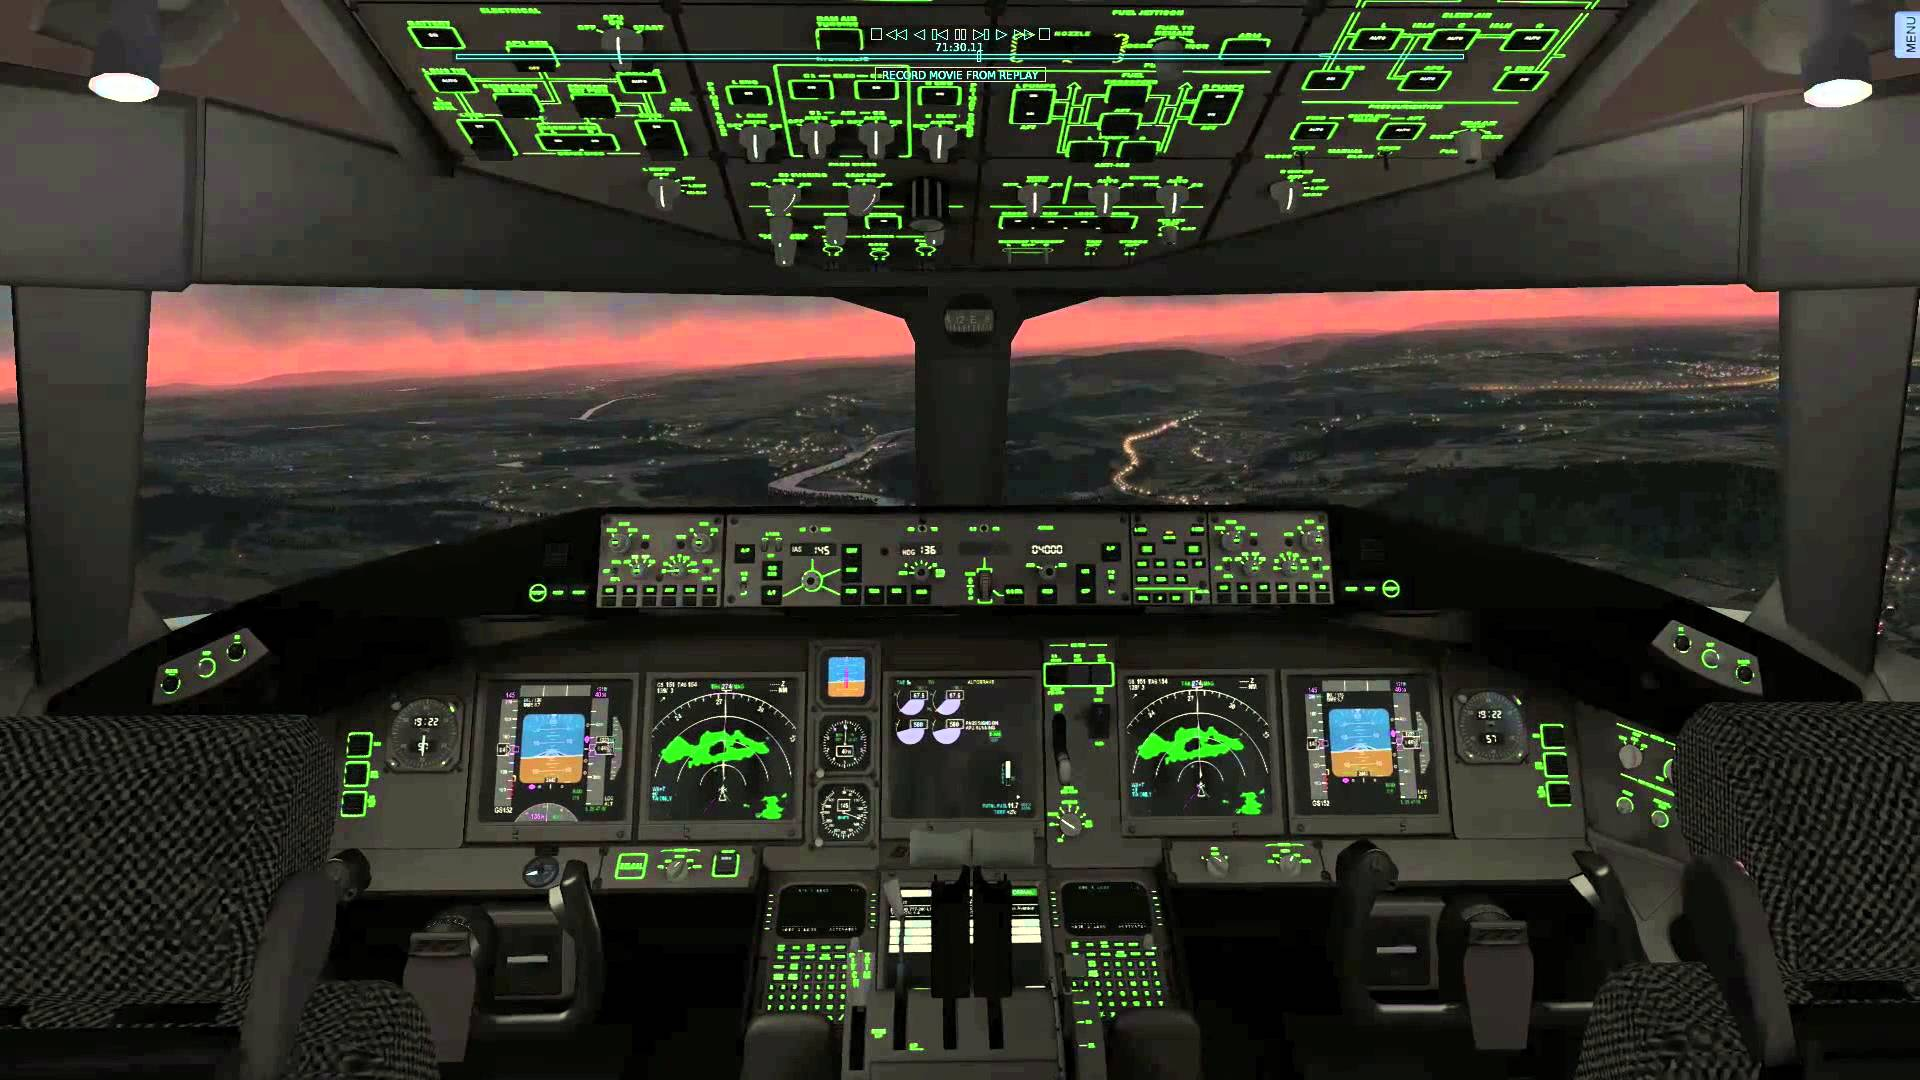
\includegraphics[width=0.8\linewidth]{figs/xplane}\\
		\tiny \href{https://www.youtube.com/watch?v=JrIu9rkAcyQ}{(Source)}
 	   \column{.5\textwidth}
	   \tiny
	   \begin{center}
	    \vspace{-0.2cm}
		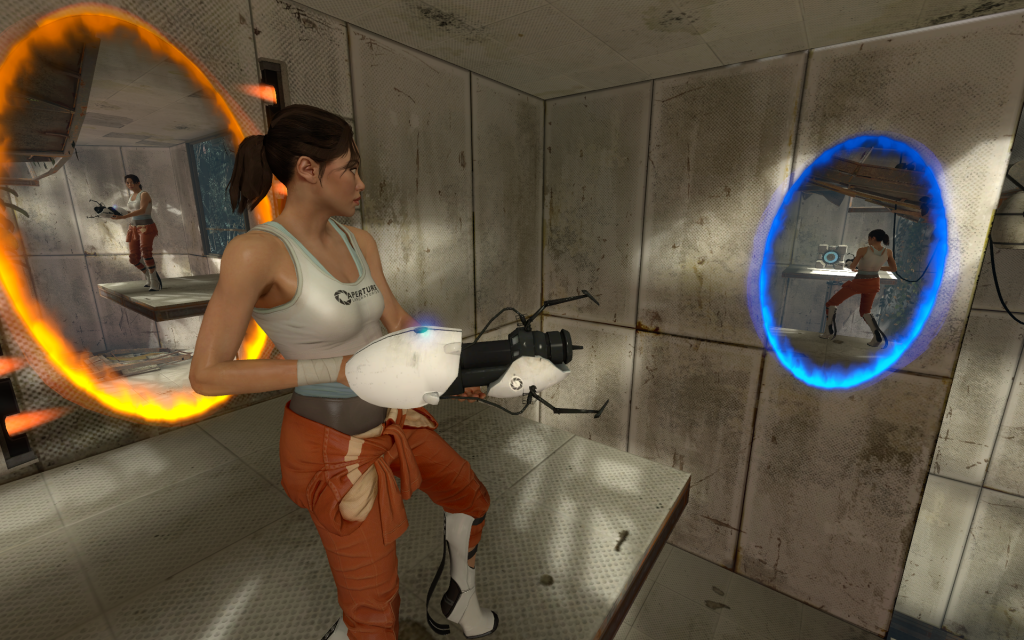
\includegraphics[width=0.8\linewidth]{figs/portals}\\
		\href{http://iagames.es/portal-survive-corto-de-accion-del-prestigioso-videojuego/}{(Source)}\\
		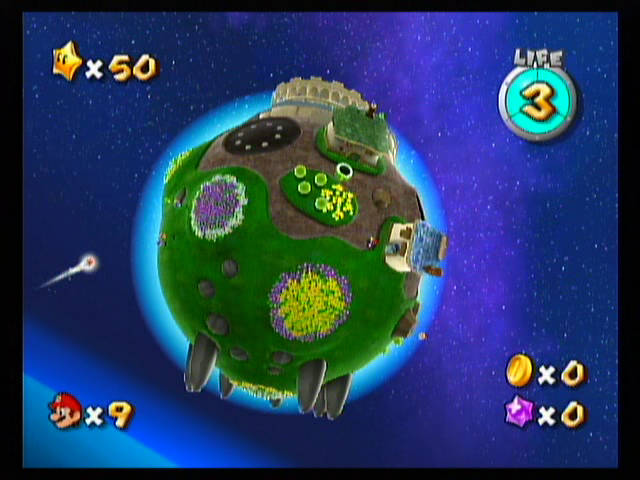
\includegraphics[width=0.8\linewidth]{figs/mariogalaxy}\\
		\href{https://s-media-cache-ak0.pinimg.com/originals/8c/f4/29/8cf429601578a742de966e985199e89e.jpg}{(Source)}
		\end{center}
	\end{columns}
\end{frame}


\subsection[Main loop]{Main loop}
\begin{frame}{Game concept}{Main loop (I)}
	%\begin{itemize}
	%\item Most videogames are graphical applications with real-time rendering
	%\end{itemize}

	Any game is based on a \alert{main loop} (or game loop)
	\begin{enumerate}
		\item Game state update
		\item Game rendering
		\item Wait
		\item Go to 1
	\end{enumerate}

	\vspace{0.2cm}
	\centering
	\begin{tikzpicture}[scale=1, auto]
	%\draw[help lines] (-2,-2) grid (6,2);

	\usetikzlibrary{shapes.misc, positioning}

	\node (init) at (-1, 0) {};
	\node (startup) [rounded rectangle, draw] at (1,0) {Startup};
	\node (update) [rounded rectangle, draw] at (3,0) {Update};
	\node (shutdown) [rounded rectangle, draw] at (6,0) {Shutdown};
	\node (draw) [rounded rectangle, draw][below of= update] {Render};


	\draw [->] (init) to node {\footnotesize{Run}} (startup);
	%\draw [->] (init.east) -- (startup.west) {hola};
	\draw [->] (startup) to node {} (update);
	\draw [->] (update) to node {\footnotesize{Finish}} (shutdown);
	\draw [->] (update.south west) -- (draw.north west);
	\draw [<-] (update.south east) -- (draw.north east);
	\end{tikzpicture}

	Not all subsystems must be run in each iteration!
\end{frame}

\begin{frame}[plain]{Game concept}{Main loop (II): Main game loop with Slick2D}
	\vspace{-0.2cm}
	\begin{block}{}
		\vspace{-0.2cm}
		\lstinputlisting[language=java, basicstyle=\ttfamily\scriptsize]{code/SlickLoop.java}
	\end{block}
\end{frame}

\begin{frame}[plain]{Game concept}{Main loop (III): Main game loop with Arcade}
	\vspace{-0.2cm}
	\begin{block}{}
		\vspace{-0.2cm}
		\lstinputlisting[language=Python, basicstyle=\ttfamily\scriptsize]{code/arcade.py}
	\end{block}

	\href{https://github.com/pvcraven/arcade/blob/master/arcade/application.py\#L36}{(Source code)}
\end{frame}

\subsection[Frame rate]{Frame rate}
\begin{frame}{Game concept}{Frame rate (I)}
	\begin{itemize}
	\item The main loop must be executed with a certain frequency
		\begin{itemize}
		\item High enough to generate an inmersive (realistic) experience
		\item Low enough not to waste computational resources
		\end{itemize}
	\item The main loop frequency determines the \textbf{Frame rate} (fps)
		\begin{itemize}
		\item The higher fps, the higher realism (and computation)
		\item 30 fps is considered as sufficient
		\item Nowdays, moving to 120 fps on new generation consoles
		\end{itemize}
	\item If the hardware is not able to maintain the given fps, the game suffers slowdown
	\end{itemize}
	\href{https://youtu.be/PLhPvS0hZSs?t=1m21s}{(Video 1)} \href{https://youtu.be/AwnQ6qF8Ots?t=1m38s}{(Video 2)} 
\end{frame}

\begin{frame}{Game concept}{Frame rate (II)}
	\begin{itemize}
	\item A trade-off is needed: fps versus game realism
	\item Complex computational models reduce fps
		\begin{itemize}
		\item Graphical components (mostly)
		\item Physics
		\item AI
		\end{itemize}
	\item Highly realistic models of the real world is not practical
	\item Videogames use simplified mathematical models
		\begin{itemize}
		\item Simplified physics
		\item Simplified NPC interation
		\end{itemize}
	\item Tricks to reduce computational needs
		\begin{itemize}
		\item Different strategies on 2D/3D games
		\item Videogame programming $\Rightarrow$ ``Tricks programming''
		\end{itemize}
	\end{itemize}
\end{frame}

\begin{frame}{Game concept}{Frame rate: Tricks (II)}
		\vspace{-0.7cm}
    \begin{columns}
   	 	\column{.50\textwidth}
		\begin{center}
			2D - Sprites\\
		    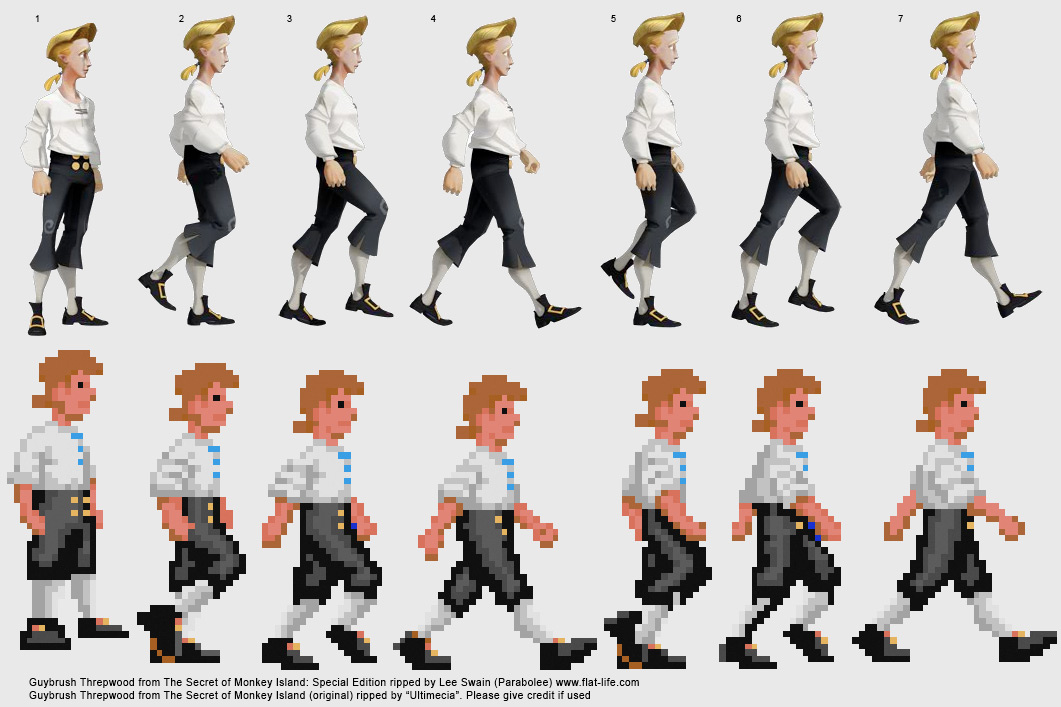
\includegraphics[width=0.9\linewidth]{figs/sprites.jpg}\\
			\smallskip
			3D - Polygons\\
		    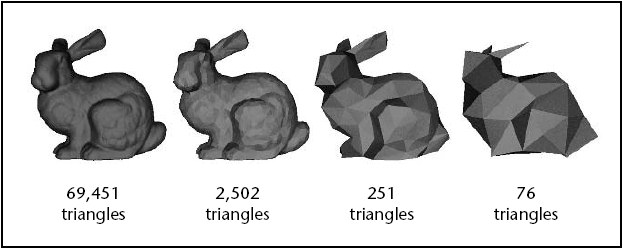
\includegraphics[width=0.9\linewidth]{figs/lod1}\\
			\smallskip
		\end{center}

 	   \column{.50\textwidth}
	   	\smallskip
		\begin{center}
	    	Level of Detail (LOD)\\
		    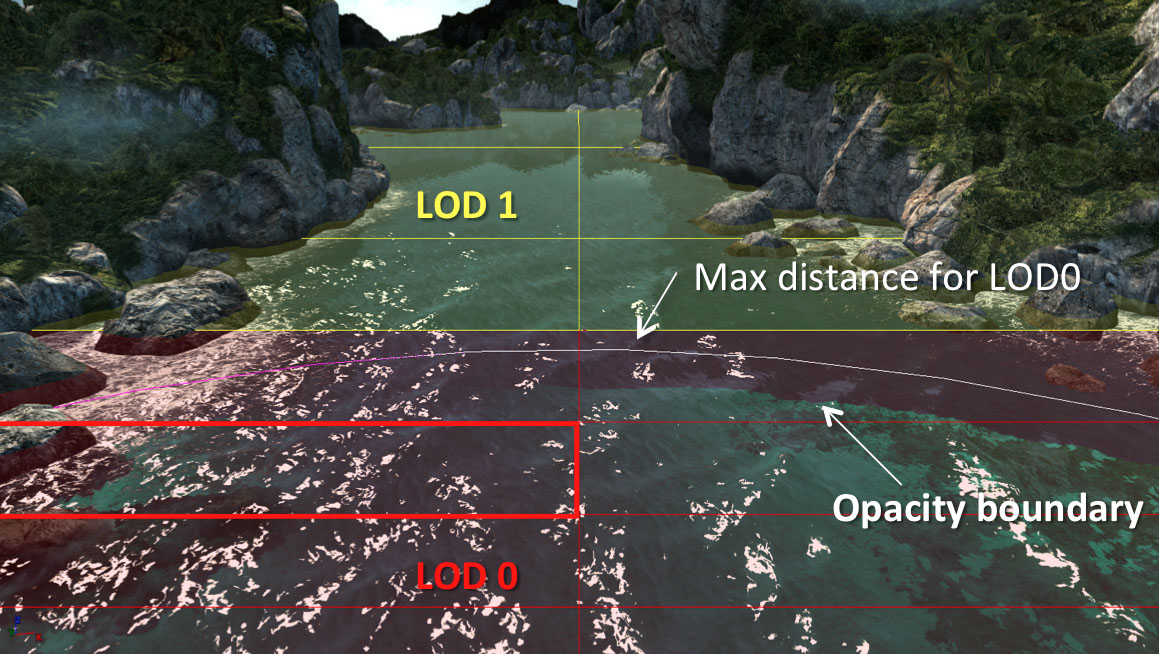
\includegraphics[width=\linewidth]{figs/lod2}\\
			\tiny{\href{http://www.fxguide.com/featured/assassins-creed-iii-the-tech-behind-or-beneath-the-action/}{(Source)}}
		    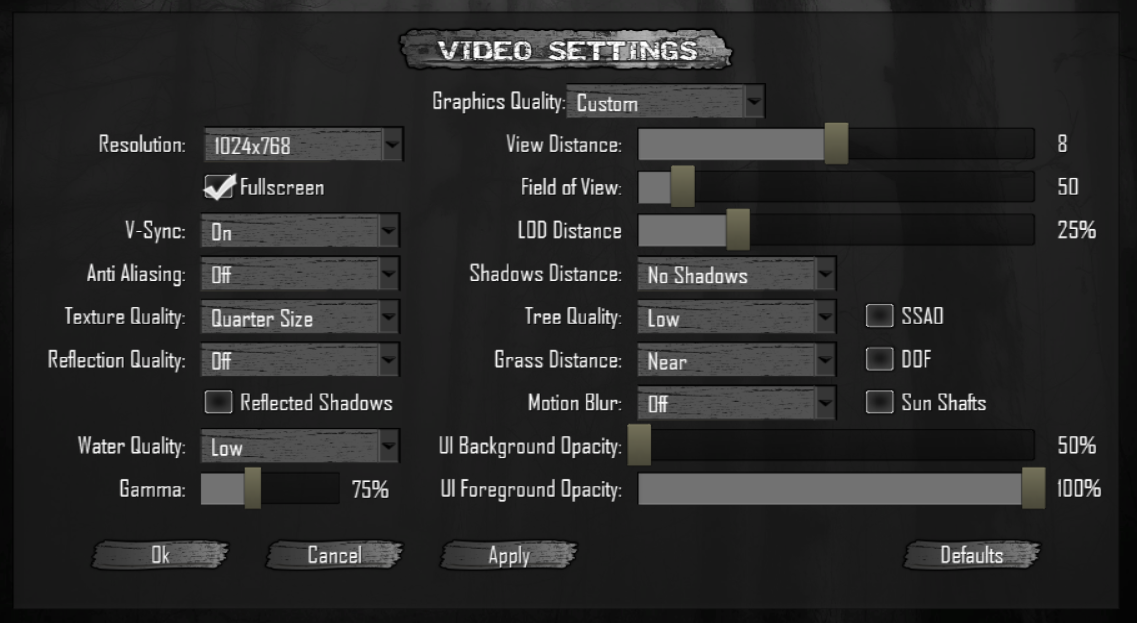
\includegraphics[width=\linewidth]{figs/lod}\\
		\end{center}
    \end{columns}

\end{frame}

\begin{frame}{Game concept}{Frame rate: Tricks (II)}
    \begin{columns}
 	   \column{.50\textwidth}
	   \smallskip
		\begin{center}
	        Fog\\
		    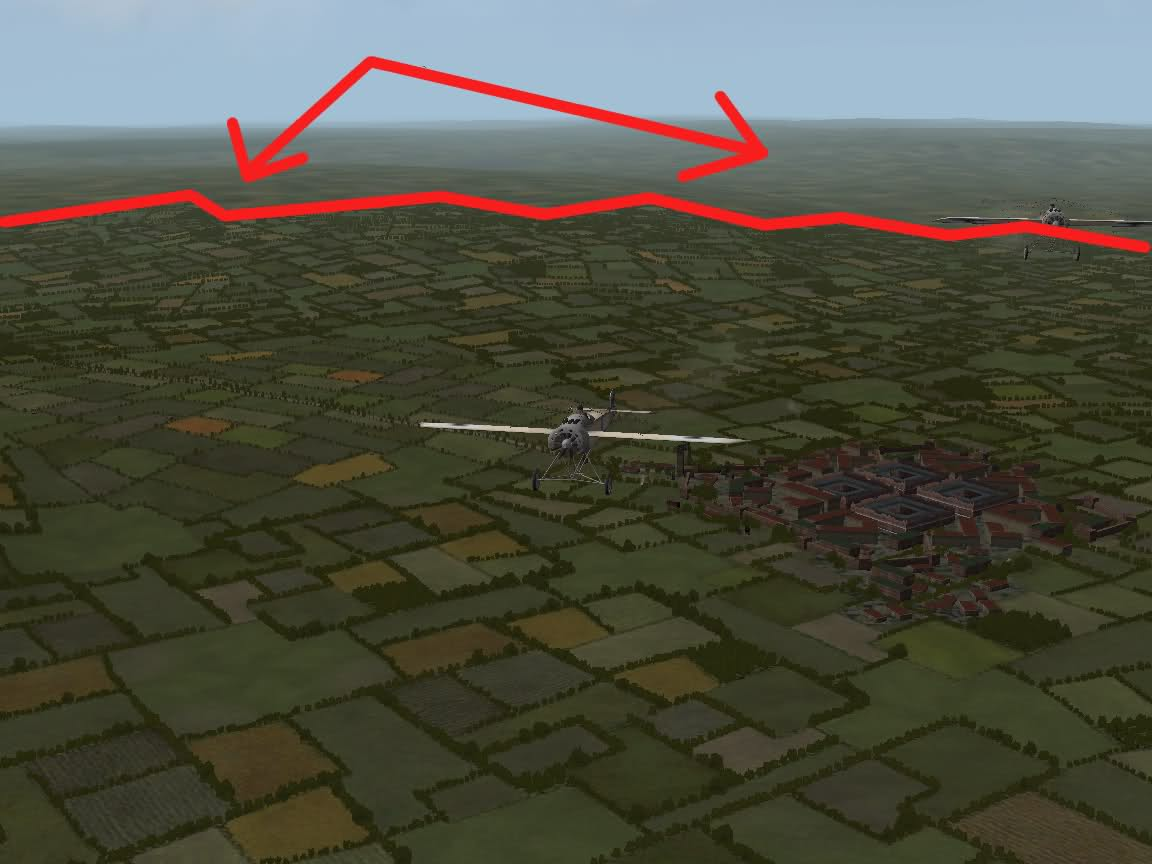
\includegraphics[width=0.8\linewidth]{figs/fog}\\
			\tiny\href{http://combatace.com/topic/50040-greatly-reduce-the-ugly-horizon-band/}{(Source)}
		\end{center}

   	 	\column{.50\textwidth}
		\begin{center}
	   		Culling\\
		    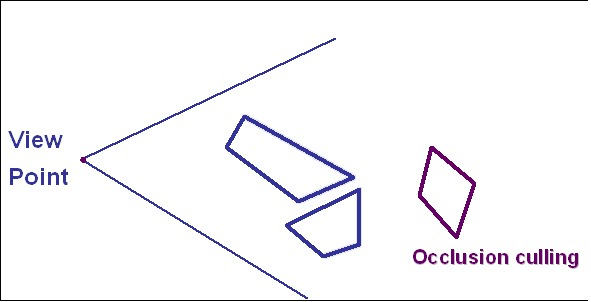
\includegraphics[width=0.7\linewidth]{figs/culling}\\
			\smallskip
	   		Clipping\\
		    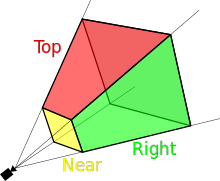
\includegraphics[width=0.7\linewidth]{figs/clipping}\\
			\bigskip
		\end{center}
    \end{columns}
\end{frame}

\section{Videogame engine}
\subsection{History}
\begin{frame}{Videogame engine}{History (I)}
    \begin{columns}
 	   \column{.70\textwidth}
	The first videogame engine emerged in the mid-nineties with \textbf{Doom}
	\begin{itemize}
		\item Doom is a classic first-person shooter \href{http://www.youtube.com/watch?v=1BkjgGTvb8s}{(Video)}
		\item Created by id Software under the supervision of \textit{John Carmack}
		\item \href{http://www.ionlitio.com/historia-id-software-los-dos-johns/}{(History of Id Software)}
	\end{itemize}
   	 \column{.30\textwidth}
   	 	\begin{figure}[t]
		\begin{center}
		    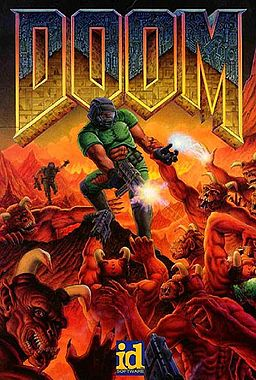
\includegraphics[width=0.7\linewidth]{figs/doom}\\
			\bigskip
		\end{center}
   	 	\end{figure}
    \end{columns}
\end{frame}

\begin{frame}{Videogame engine}{History (II)}
	\begin{itemize}
	\item Doom was designed using a reuse-oriented architecture
	\item The architedture was based on several modules
		\begin{itemize}
		\item Rendering
		\item Collision detection
		\item Audio
		\item Artistic components (i.e., levels)
		\item Rule system that controls the game
		\end{itemize}
		\end{itemize}
	\vspace{-0.4cm}
    \begin{columns}
 	   \column{.32\textwidth}
   	 	\begin{figure}[t]
		\begin{center}
		    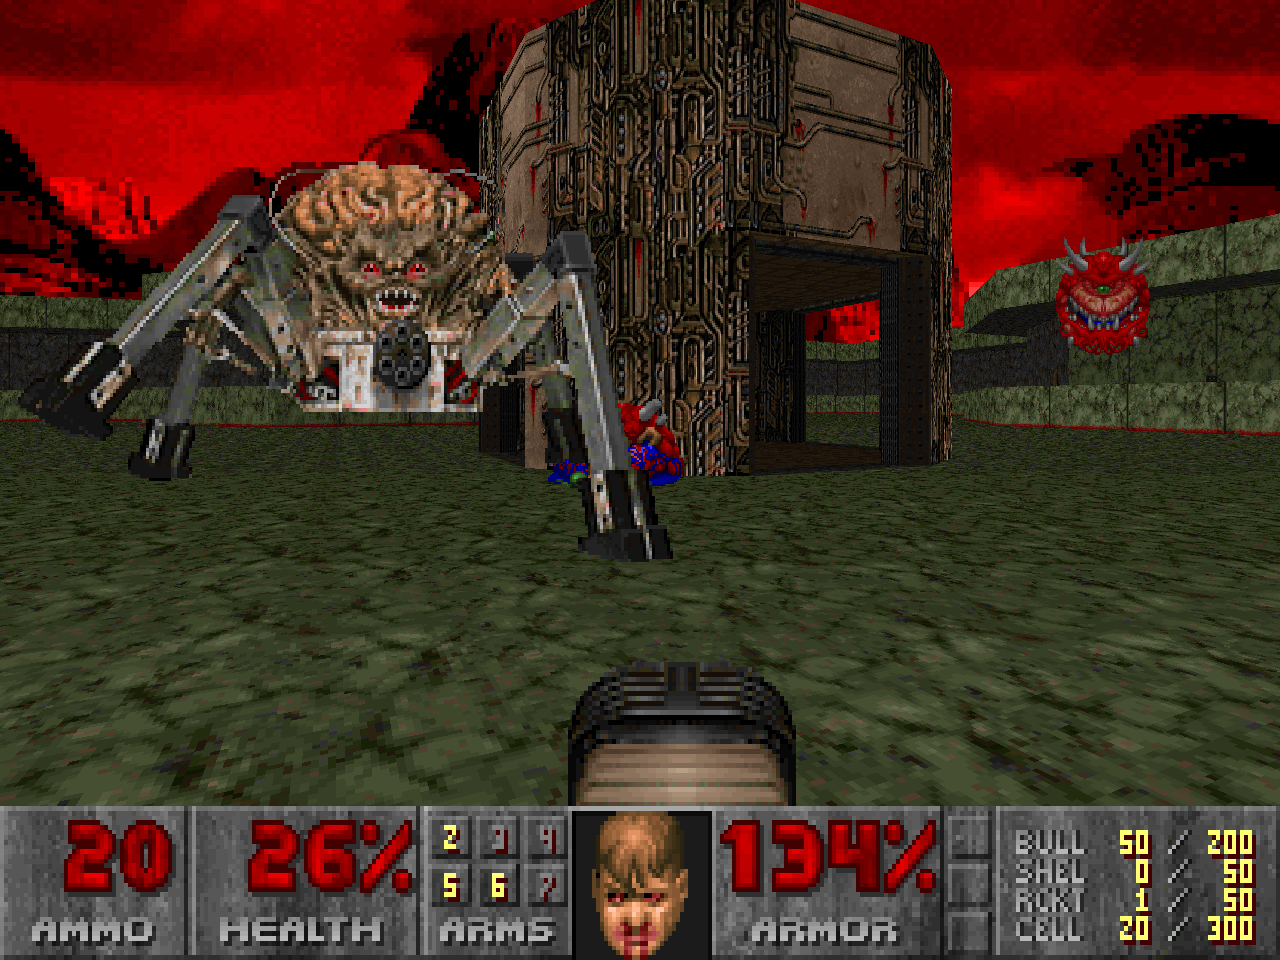
\includegraphics[width=\linewidth]{figs/doom1}\\
			Doom 1
			\bigskip
		\end{center}
   	 	\end{figure}
		\column{.32\textwidth}
   	 	\begin{figure}[t]
		\begin{center}
		    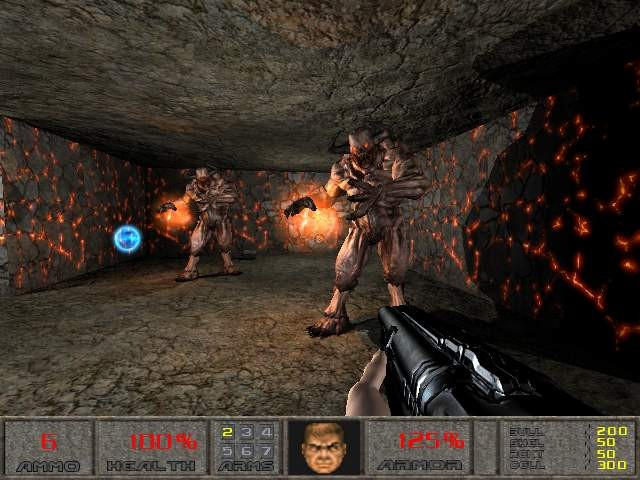
\includegraphics[width=\linewidth]{figs/doom2}\\
			Doom 2
			\bigskip
		\end{center}
   	 	\end{figure}
		\column{.32\textwidth}
   	 	\begin{figure}[t]
		\begin{center}
		    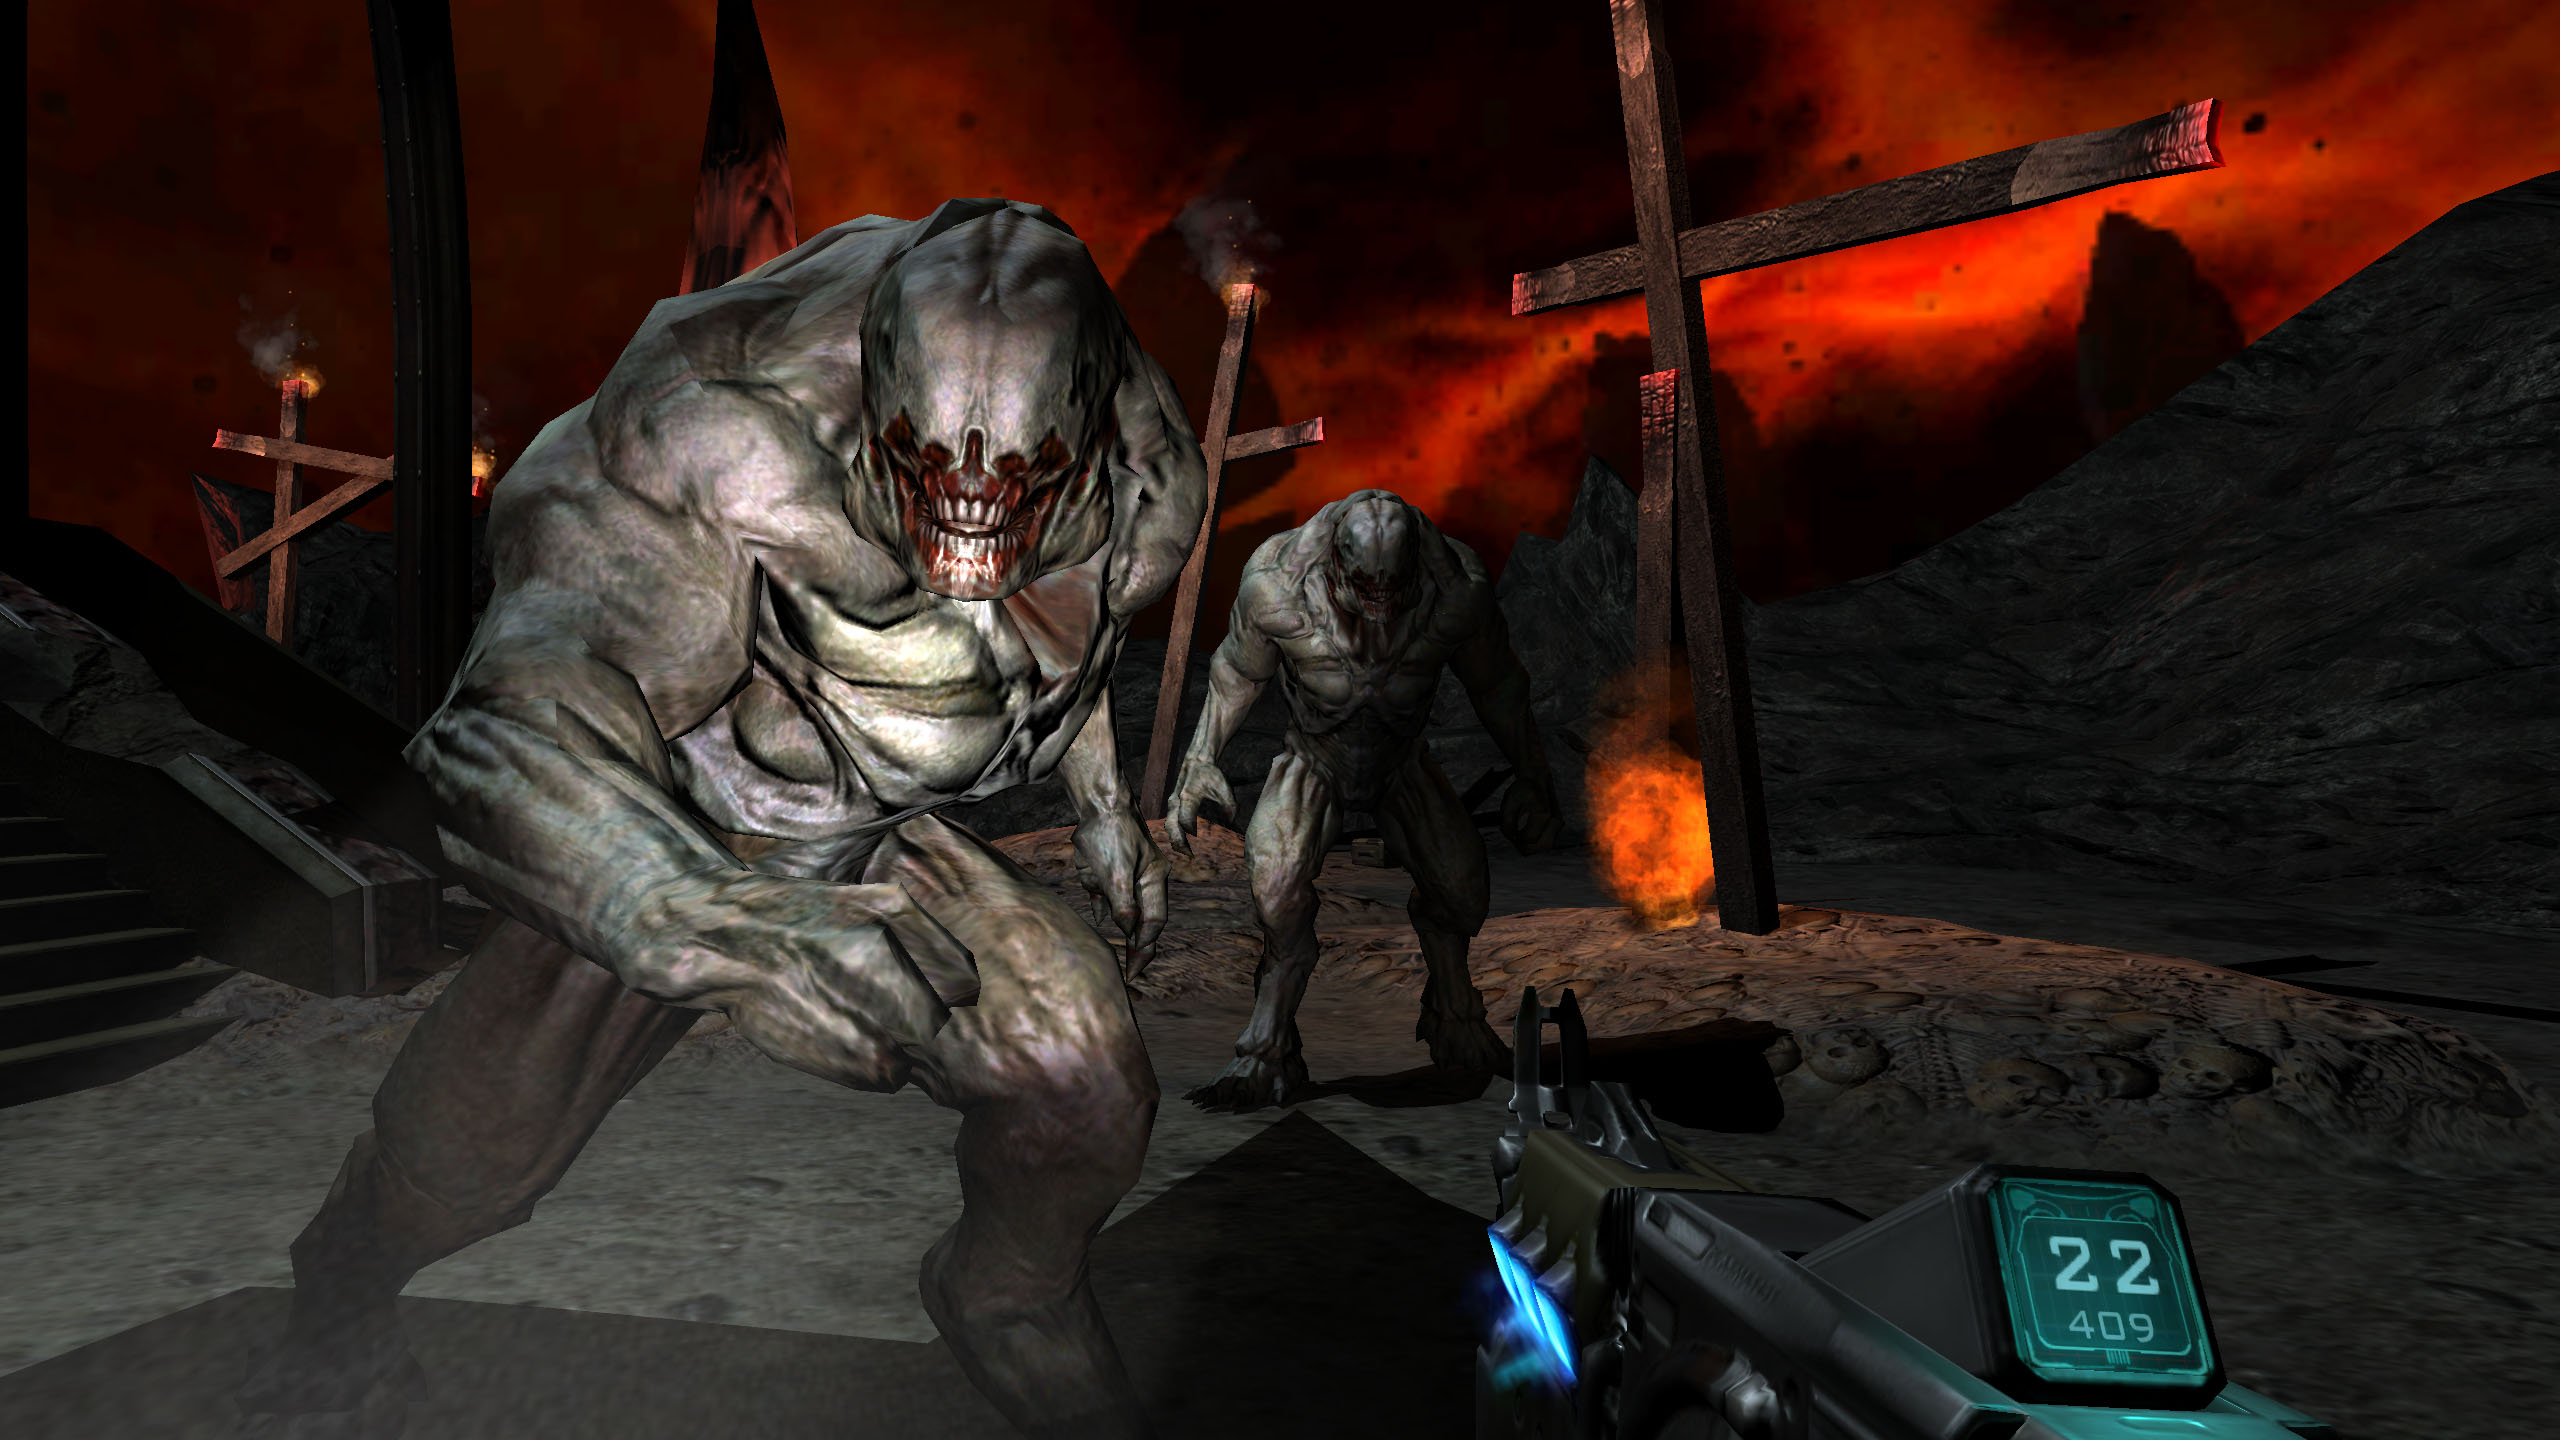
\includegraphics[width=\linewidth]{figs/doom3}\\
			Doom 3
			\bigskip
		\end{center}
   	 	\end{figure}
	\end{columns}
\end{frame}

\subsection{Definition}
\begin{frame}{Videogame engine}{Definition (I)}
	\vspace{-0.1cm}
	\begin{block}{Videogame engine}
	The videogame engine is a tool that ease game development by means of task automation and hidding some low-level issues
	\end{block}

	\vspace{-0.1cm}
	\begin{itemize}
		\item The main goal of any videogame engine is code re-use
		\item Videogame of the \textbf{same type} with almost no engine coding
		\begin{itemize}
		\item Development can focus on art design and game rules
		\end{itemize}
	\end{itemize}

	\vspace{-0.2cm}
    \begin{columns}
 	   \column{.1\textwidth}
 	   \column{.4\textwidth}
   	 	\begin{figure}[t]
		\begin{center}
		    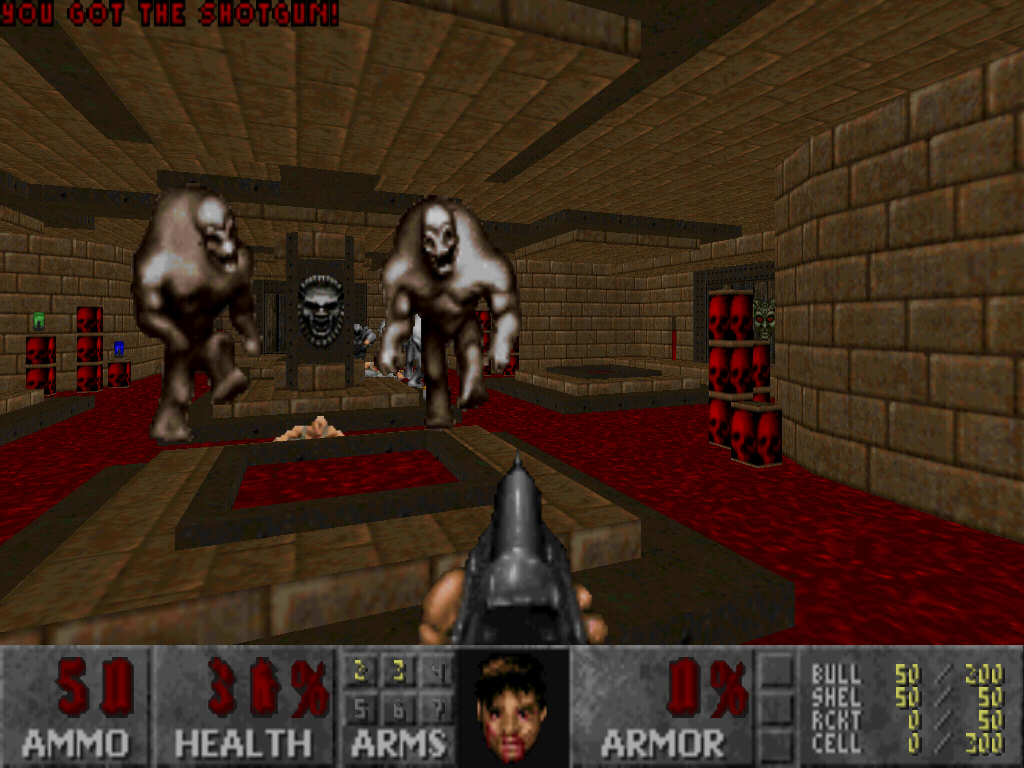
\includegraphics[width=0.8\linewidth]{figs/freedoom}\\
			Freedoom
			\bigskip
		\end{center}
   	 	\end{figure}
		\column{.4\textwidth}
   	 	\begin{figure}[t]
		\begin{center}
		    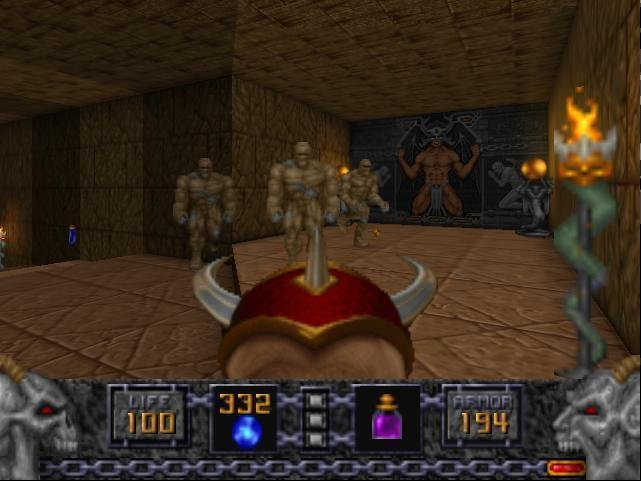
\includegraphics[width=0.8\linewidth]{figs/heretic}\\
			Heretic
			\bigskip
		\end{center}
   	 	\end{figure}
 	   \column{.1\textwidth}
	\end{columns}
\end{frame}

\begin{frame}{Videogame engine}{Definition (II)}
	Decoupling the engine and the videogame is not possible
	\begin{itemize}
		\item It limits the complete reuse of the engine
	\end{itemize}
	The main dependence is the game genre
	\begin{itemize}
		\item Different genres involves different needs
	\end{itemize}
	Some low level modules are easier to generalize
	\begin{itemize}
		\item User events, audio, text rendering, ...
	\end{itemize}
	\textit{Game engine tuning}: Capacity of videogame engine to adapt and satisfy specific needs
\end{frame}


\subsection{Commercial engines}
\begin{frame}{Videogame engine}{Commercial engines (I)}
	\vspace{-0.2cm}
    \begin{columns}
 	   \column{.4\textwidth}
		\vspace{-0.2cm}
   	 	\begin{figure}[t]
		\begin{center}
		    
\includegraphics[width=0.8\linewidth]{figs/unreal}\\
			\small{BioShock, Gears of War\\
			\href{https://en.wikipedia.org/wiki/List_of_Unreal_Engine_games}{(List of games)}}

		    
\includegraphics[width=0.8\linewidth]{figs/CRYENGINE}\\
			\small{Far Cry, Crysis\\
			\href{https://en.wikipedia.org/wiki/List_of_CryEngine_games}{(List of games)}
			}
		\end{center}
   	 	\end{figure}
		\column{.4\textwidth}
		\vspace{-0.3cm}
   	 	\begin{figure}[t]
		\begin{center}
		    
\includegraphics[width=0.8\linewidth]{figs/unity}\\
			\small{Angry Birds 
			\href{https://en.wikipedia.org/wiki/List_of_Unity_games}{(List of games)}
			}
		
			\bigskip

		    
\includegraphics[width=0.8\linewidth]{figs/frostbite}\\
			\small{Battlefield, Need for Speed\\
			\href{https://en.wikipedia.org/wiki/List_of_Frostbite_games}{(List of games)}
			}
			\end{center}
   	 	\end{figure}
	\end{columns}
	\begin{center}
		    
\includegraphics[width=0.3\linewidth]{figs/source}\\
			\small{Half Life \href{https://en.wikipedia.org/wiki/Source_(game_engine)}{(List of games)}}
	\end{center}
\end{frame}

\begin{frame}{Videogame engine}{Commercial engines (II)}
	\vspace{-0.2cm}
    \begin{columns}
 	   \column{.4\textwidth}
		\vspace{-0.5cm}
   	 	\begin{figure}[t]
		\begin{center}
		    
\includegraphics[width=0.7\linewidth]{figs/libgdx}\\
		    
\includegraphics[width=0.5\linewidth]{figs/jmonkey}
		    
\includegraphics[width=0.45\linewidth]{figs/cocos2d1}\\
			\bigskip
		    
\includegraphics[width=0.8\linewidth]{figs/pygame_logo}\\
		\end{center}
   	 	\end{figure}
		\column{.4\textwidth}
		\vspace{-1cm}
   	 	\begin{figure}[t]
		\begin{center}
		    
\includegraphics[width=0.6\linewidth]{figs/godot}\\
			\medskip
		    
\includegraphics[width=0.8\linewidth]{figs/love}\\
			\medskip
		    
\includegraphics[width=0.8\linewidth]{figs/xna}\\
			\medskip
		    
\includegraphics[width=0.8\linewidth]{figs/slick2d}\\
		\end{center}
   	 	\end{figure}
	\end{columns}
\end{frame}

\section{Videogames genres}
\subsection[Third person videogames]{Third person videogames}
\begin{frame}{Videogames genres}{Third person videogames}
	\vspace{-0.3cm}
    \begin{columns}
 	   \column{.60\textwidth}
		Features
			\begin{itemize}
			\item Puzzles
			\item Platforms
			\item Advanced motion
			\end{itemize}
	 	Challenges
			\begin{itemize}
			\item Camera motion
			\item Camera collision detection
			\item Player cinematics
			\end{itemize}

   	 \column{.40\textwidth}
   	 	\begin{figure}[t]
		\begin{center}
		    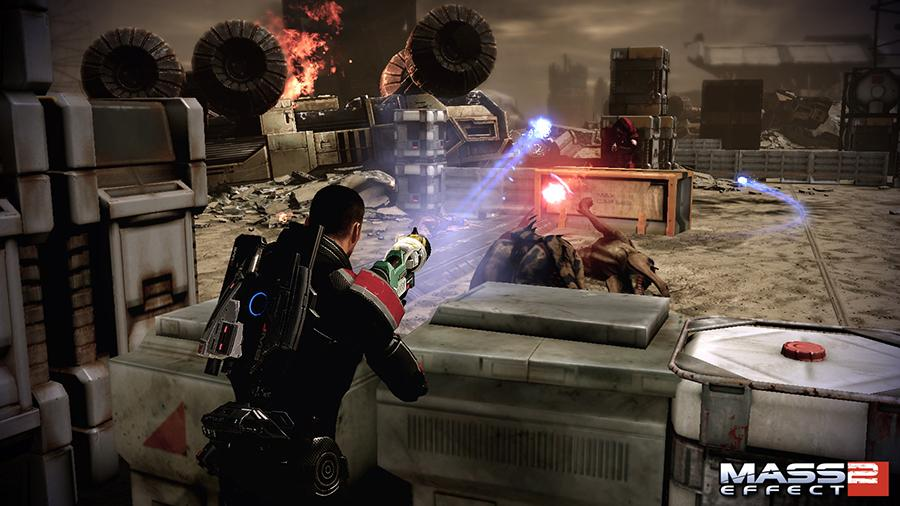
\includegraphics[width=0.9\linewidth]{figs/mass2}\\Mass effect 2\\\bigskip
		    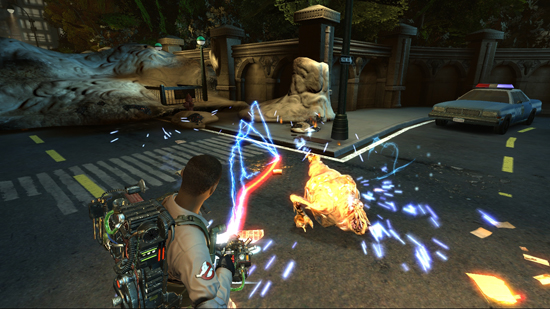
\includegraphics[width=0.9\linewidth]{figs/ghostbuster2}\\Ghostbusters 2\\
		\end{center}
   	 	\end{figure}
    \end{columns}
\end{frame}

\subsection[Fighting videogames]{Fighting videogames}
\begin{frame}{Videogames genres}{Fighting videogames}
	\vspace{-0.4cm}
    \begin{columns}
 	   \column{.60\textwidth}
		Features
			\begin{itemize}
			\item 3D environment and players
			\item 2D motion (lateral scroll)
			\item Environments with limited size
			\item Complex players animation
			\end{itemize}
	 	Challenges
			\begin{itemize}
			\item Great player graphical quality
			\item Collision detection with players and weapons
			\item Complex input (variety of attacks)
			\end{itemize}

   	 \column{.40\textwidth}
   	 	\begin{figure}[t]
		\begin{center}
		    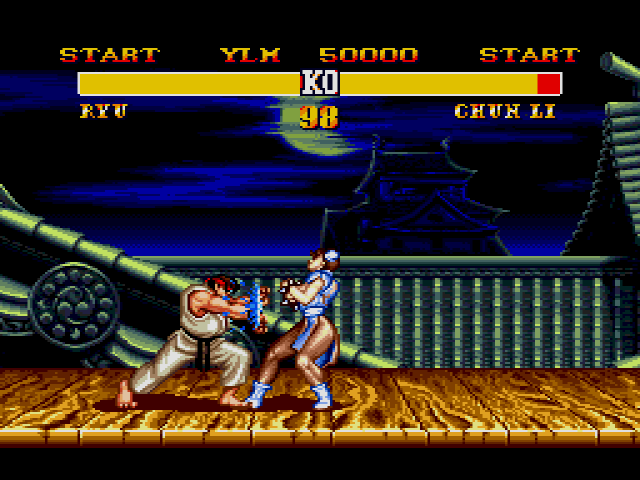
\includegraphics[width=0.9\linewidth]{figs/sf}\\Street fighter\\\smallskip
		    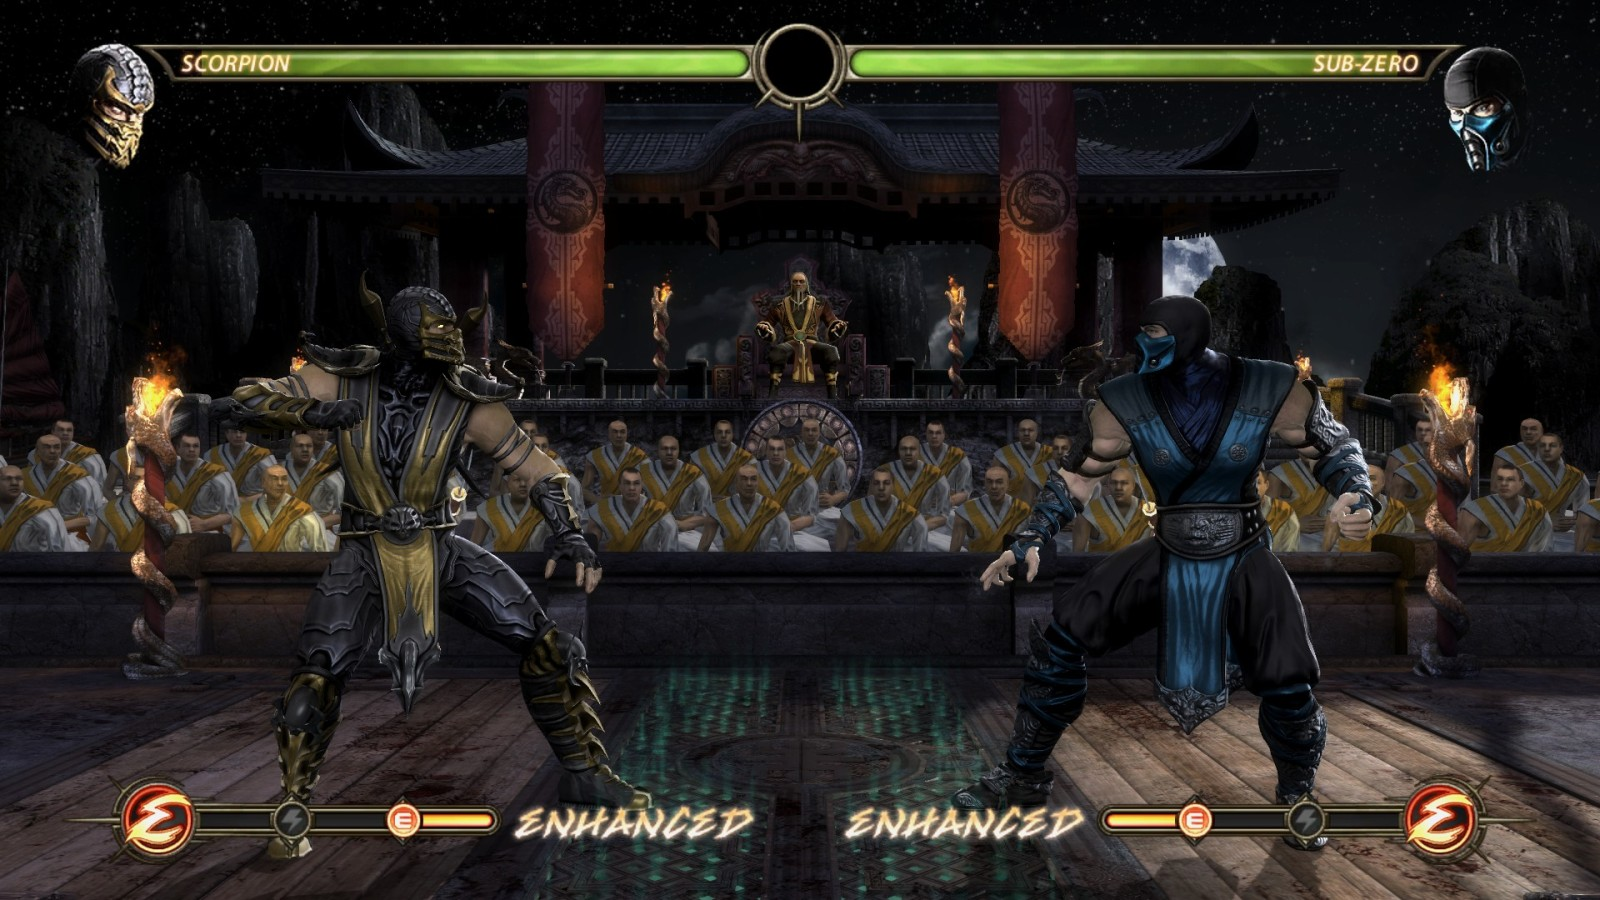
\includegraphics[width=0.9\linewidth]{figs/mortalcombat9}\\Mortal Combat 9
		\end{center}
   	 	\end{figure}
    \end{columns}
\end{frame}

\subsection[Racing videogames]{Racing videogames}
\begin{frame}{Videogames genres}{Racing videogames}
	\vspace{-0.4cm}
    \begin{columns}
 	   \column{.60\textwidth}
		Features
			\begin{itemize}
			\item Two subgenres: Simulation and arcade
			\item Related genre: Flight simulators
			\end{itemize}
	 	Challenges
			\begin{itemize}
			\item Custom hardware
			\item Physics
			\item High graphical quality
			\item Speed
			\item Create speed perception
			\end{itemize}

   	 \column{.40\textwidth}
   	 	\begin{figure}[t]
		\begin{center}
		    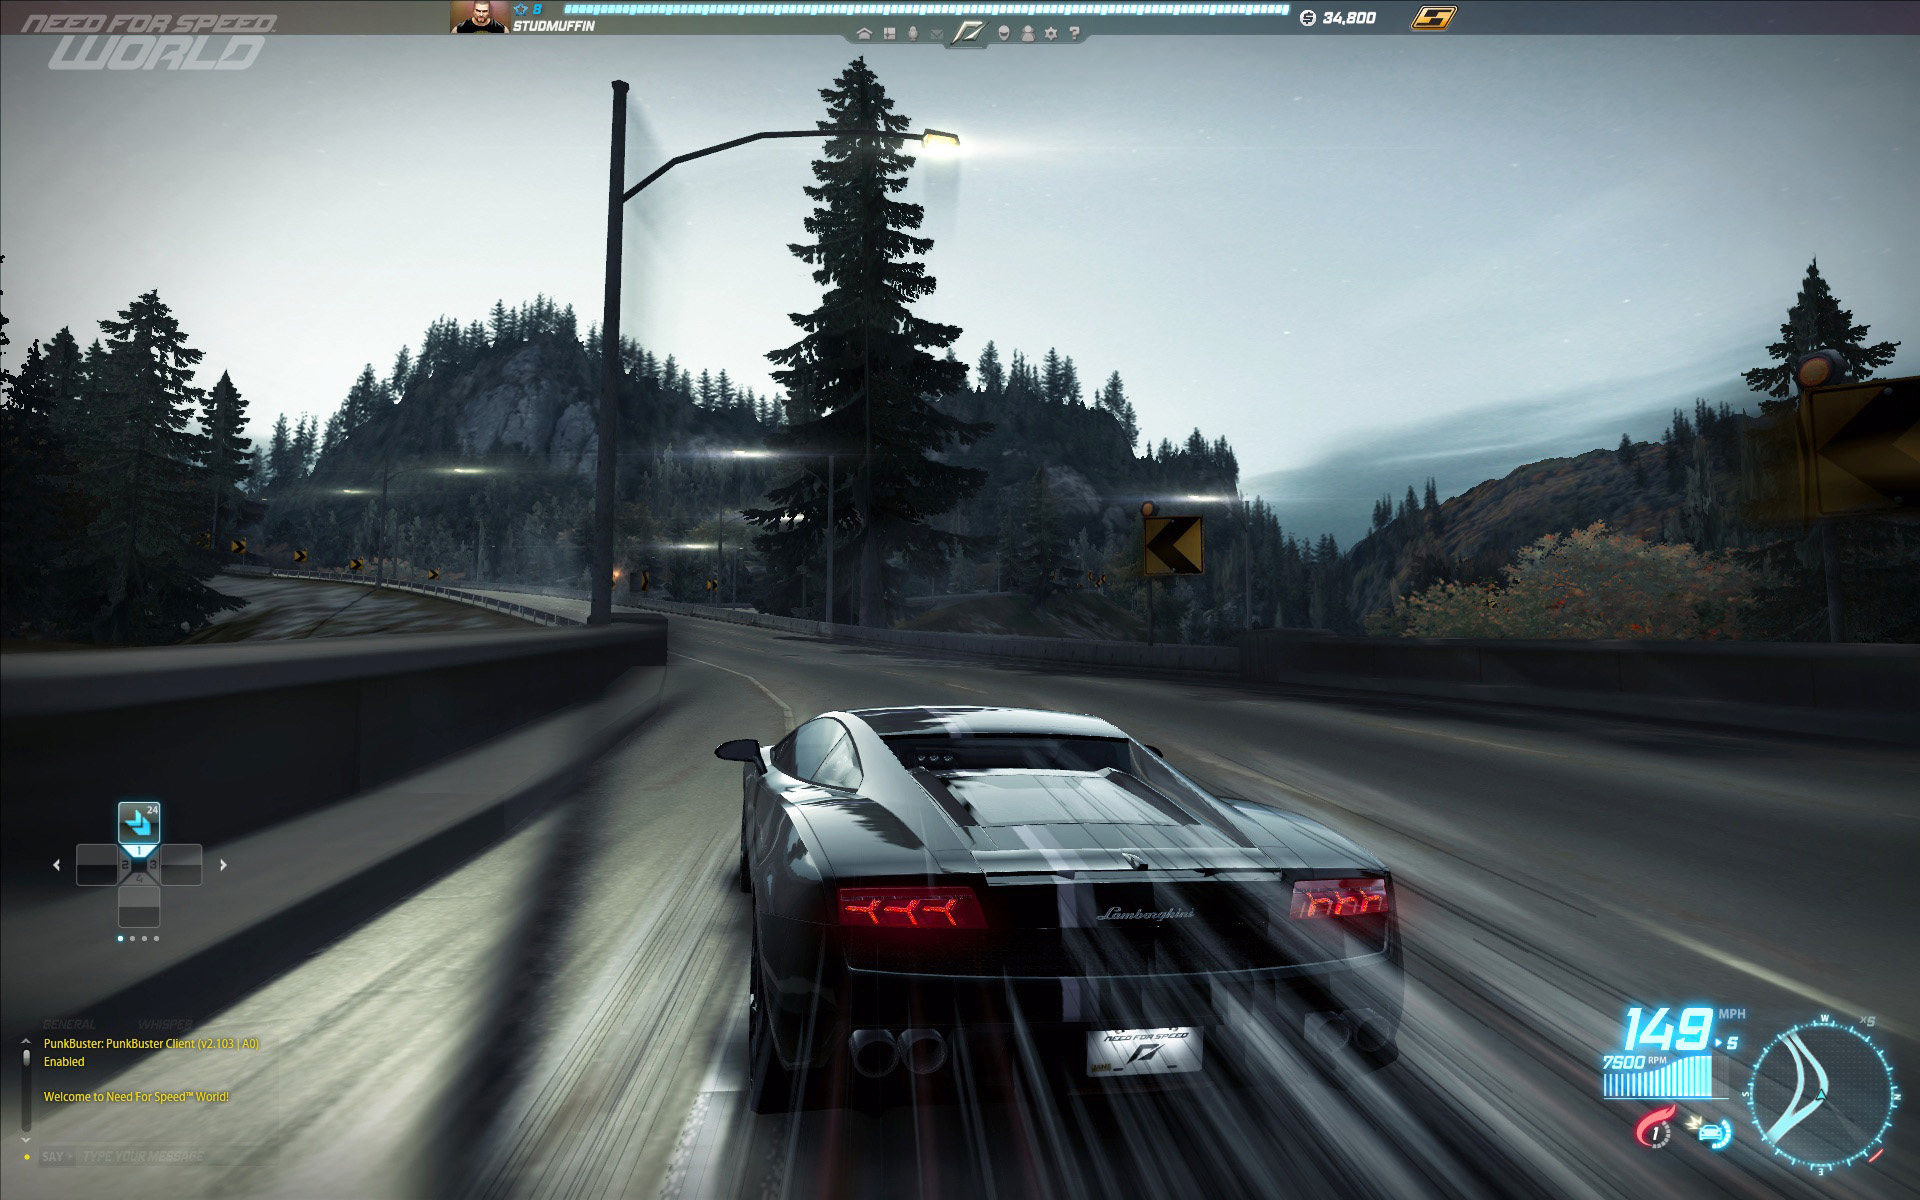
\includegraphics[width=0.9\linewidth]{figs/n4s}\\Need for speed\\\smallskip
		    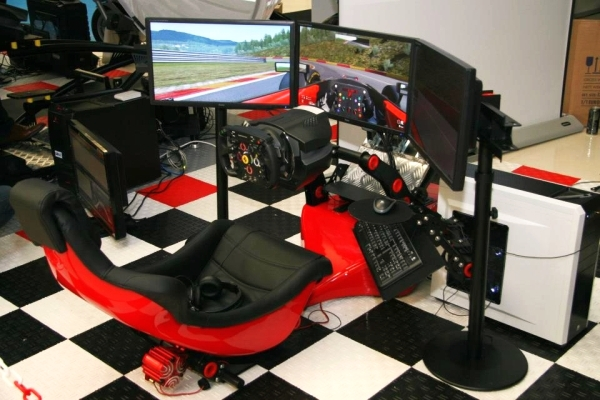
\includegraphics[width=0.9\linewidth]{figs/f1}
		\end{center}
   	 	\end{figure}
    \end{columns}
\end{frame}

\subsection{Strategy}
\begin{frame}{Videogames genres}{Strategy}
	\vspace{-0.4cm}
    \begin{columns}
 	   \column{.60\textwidth}
		Features
			\begin{itemize}
			\item Two subgenres: Real-time and turn-based strategy
			\item Isometric view
			\item 2D or 3D environments		
			\item Low resolution players
			\end{itemize}
	 	Challenges
			\begin{itemize}
			\item Large number of units
			\item Complex user interfaces
			\item AI
			\item Technology trees
			\end{itemize}

   	 \column{.40\textwidth}
   	 	\begin{figure}[t]
		\begin{center}
		    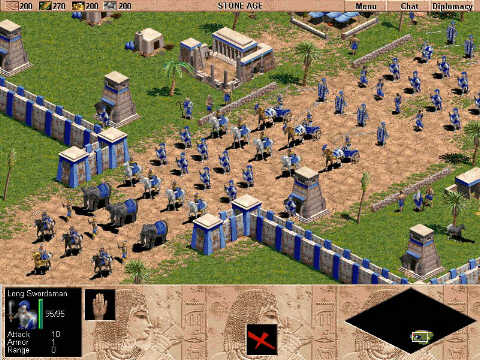
\includegraphics[width=0.9\linewidth]{figs/age-of-empires}\\Age of Empires 2\\
		    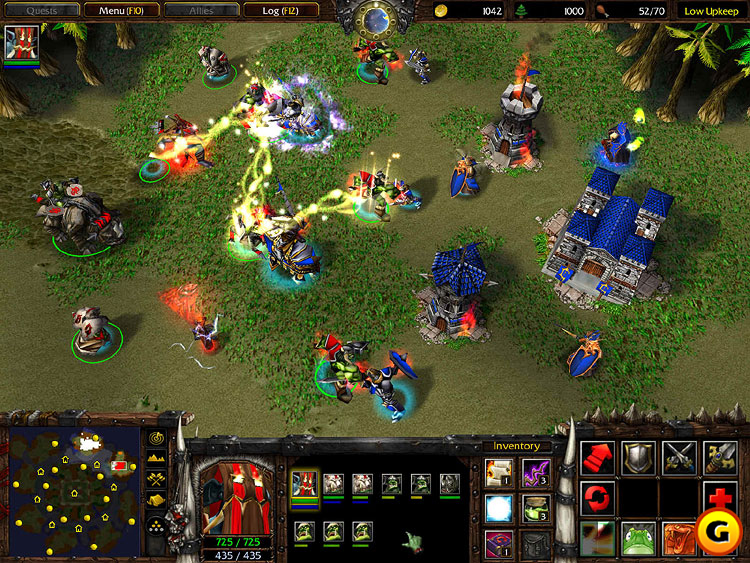
\includegraphics[width=0.9\linewidth]{figs/warcraft}\\Warcraft 3
		\end{center}
   	 	\end{figure}
    \end{columns}
\end{frame}

\subsection{Massively Multiplayer Online Game (MMOG)}
\begin{frame}{Videogames genres}{Massively Multiplayer Online Game (MMOG)}
    \begin{columns}
 	   \column{.60\textwidth}
		Features
			\begin{itemize}
			\item Large (or huge)  number of users
			\item Low resolution players
			\end{itemize}
	 	Challenges
			\begin{itemize}
			\item Intense networking usage
			\item Bussiness model	
			\end{itemize}

   	 \column{.40\textwidth}
   	 	\begin{figure}[t]
		\begin{center}
		    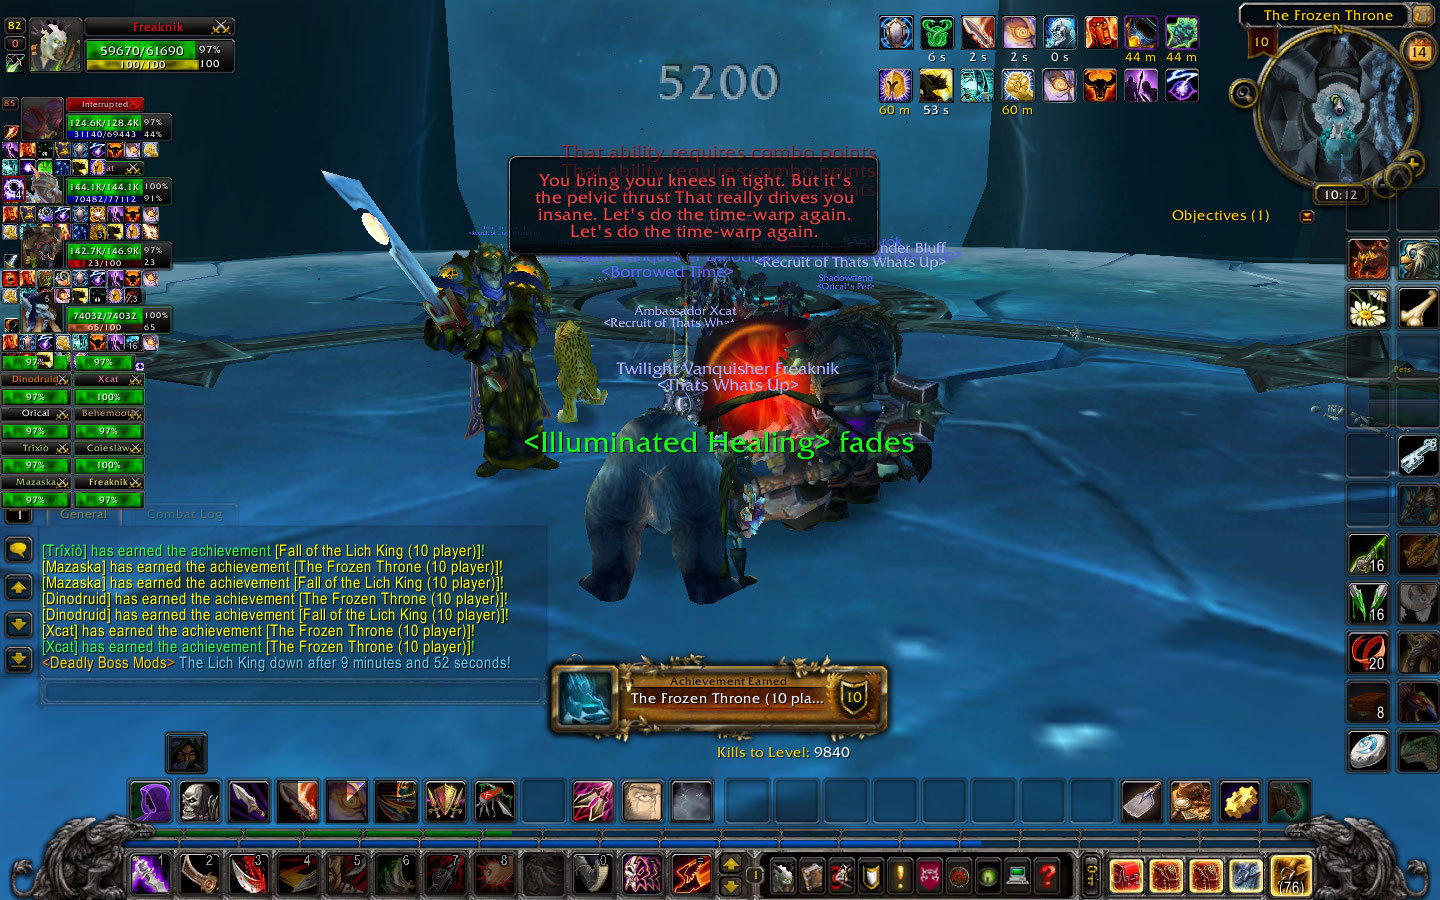
\includegraphics[width=0.9\linewidth]{figs/wow}\\World of Warcraft\\\bigskip
		    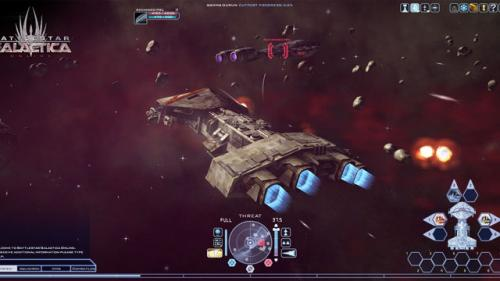
\includegraphics[width=0.9\linewidth]{figs/galactica}\\Galactica Online
		\end{center}
   	 	\end{figure}
    \end{columns}
\end{frame}

\begin{frame}{Videogames genres}{Others}
	\begin{itemize}
	\item Sports
	\item RPG
	\item Puzzles
	\item Platforms
	\end{itemize}
\end{frame}



\end{document}
